% !TEX TS-program = pdflatex
% !TEX encoding = UTF-8 Unicode
\documentclass[border=0mm]{standalone}
% packages
\usepackage{tikz}
\usetikzlibrary{patterns}
\usepackage{amsmath,amssymb}
\usepackage{bm}
\usepackage{pgfplots}
\pgfplotsset{compat=1.15}
% start document
\begin{document}
% generated by ROOT (CERN)
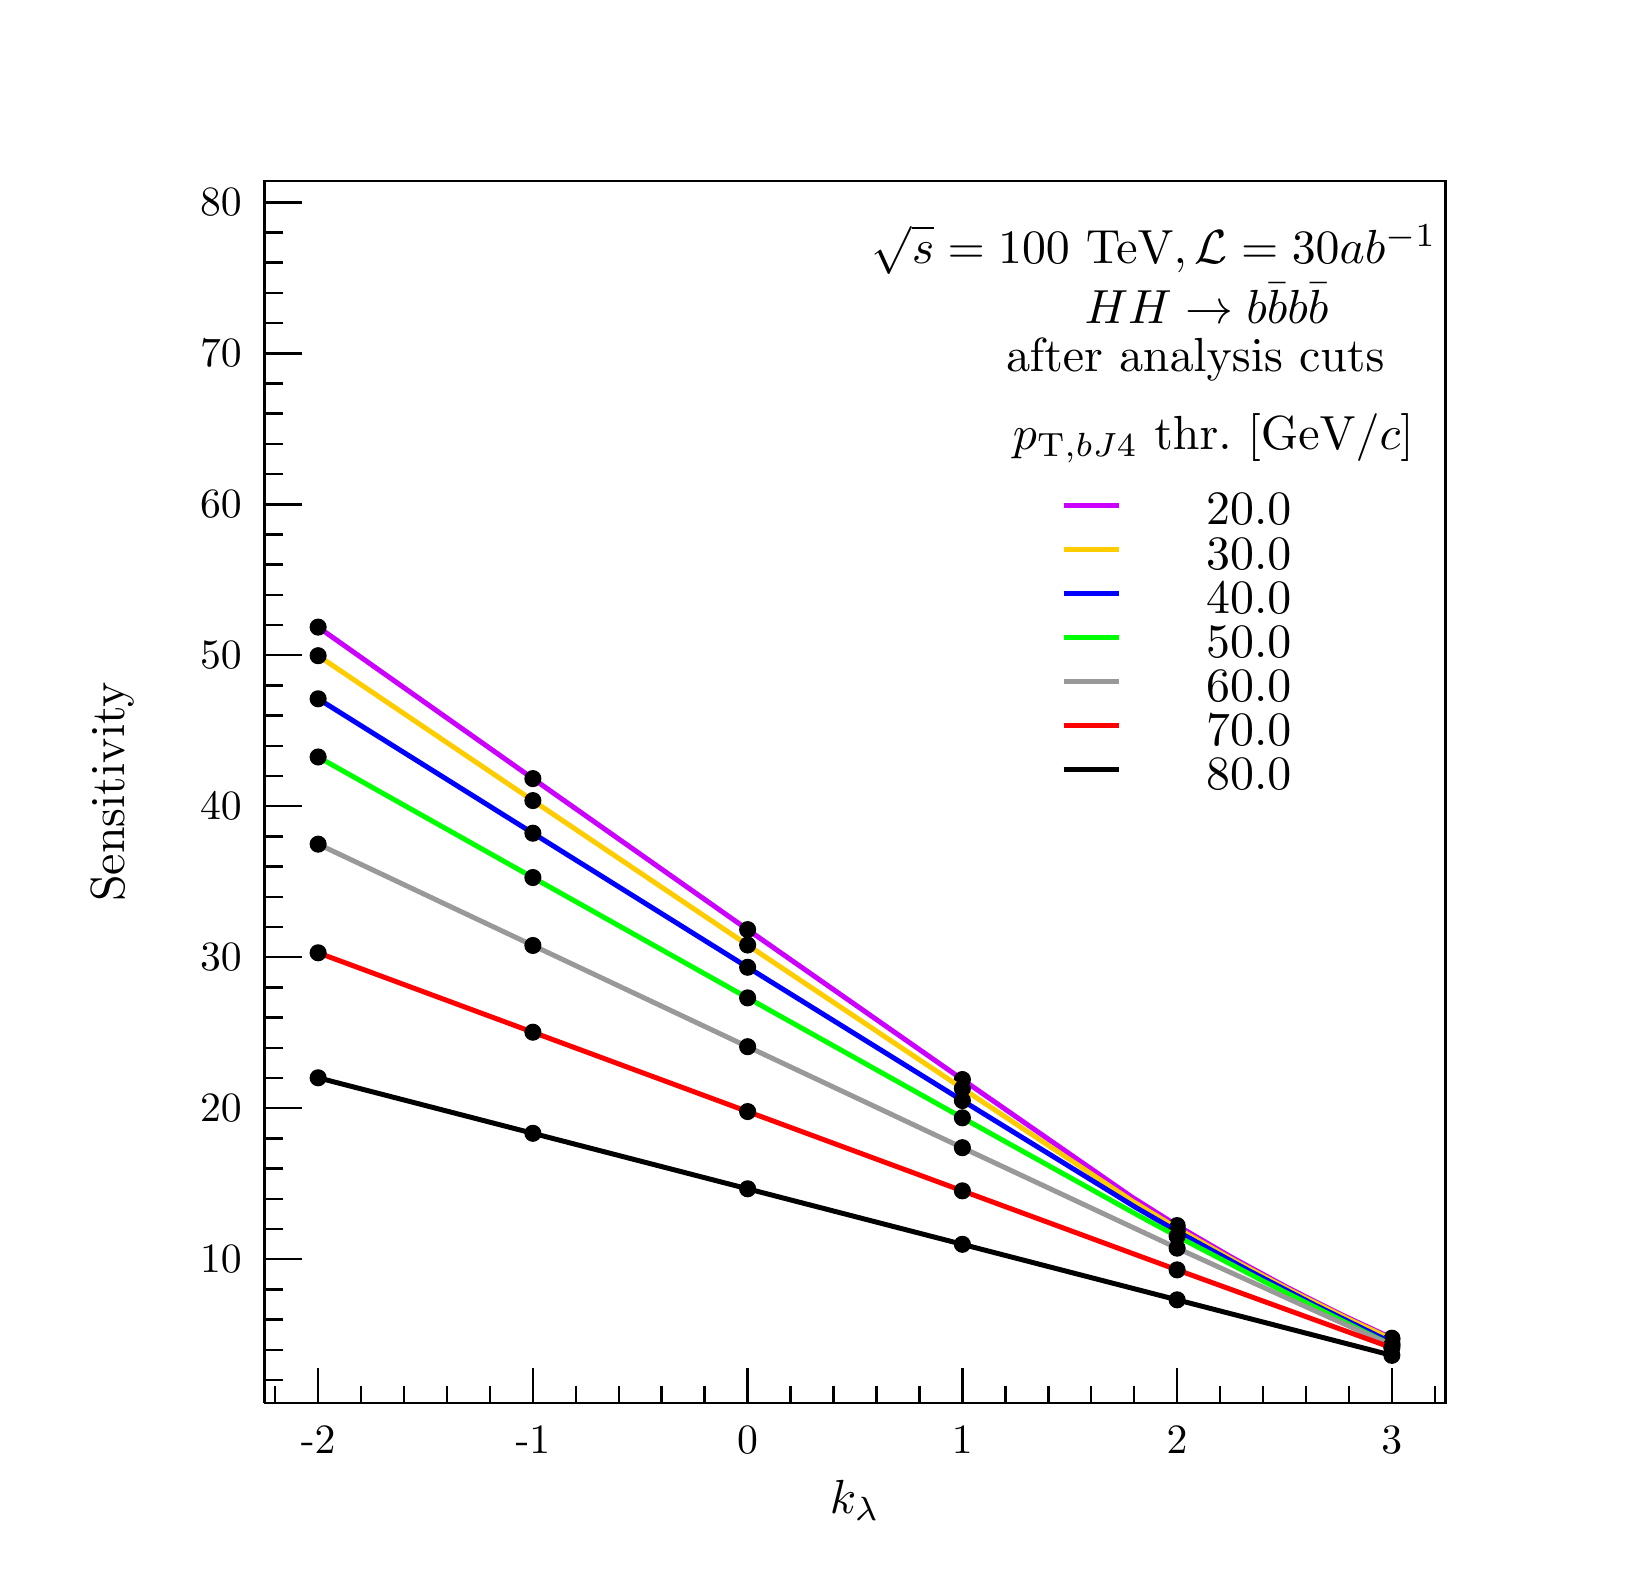
\begin{tikzpicture}
\pgfdeclareplotmark{cross} {
\pgfpathmoveto{\pgfpoint{-0.3\pgfplotmarksize}{\pgfplotmarksize}}
\pgfpathlineto{\pgfpoint{+0.3\pgfplotmarksize}{\pgfplotmarksize}}
\pgfpathlineto{\pgfpoint{+0.3\pgfplotmarksize}{0.3\pgfplotmarksize}}
\pgfpathlineto{\pgfpoint{+1\pgfplotmarksize}{0.3\pgfplotmarksize}}
\pgfpathlineto{\pgfpoint{+1\pgfplotmarksize}{-0.3\pgfplotmarksize}}
\pgfpathlineto{\pgfpoint{+0.3\pgfplotmarksize}{-0.3\pgfplotmarksize}}
\pgfpathlineto{\pgfpoint{+0.3\pgfplotmarksize}{-1.\pgfplotmarksize}}
\pgfpathlineto{\pgfpoint{-0.3\pgfplotmarksize}{-1.\pgfplotmarksize}}
\pgfpathlineto{\pgfpoint{-0.3\pgfplotmarksize}{-0.3\pgfplotmarksize}}
\pgfpathlineto{\pgfpoint{-1.\pgfplotmarksize}{-0.3\pgfplotmarksize}}
\pgfpathlineto{\pgfpoint{-1.\pgfplotmarksize}{0.3\pgfplotmarksize}}
\pgfpathlineto{\pgfpoint{-0.3\pgfplotmarksize}{0.3\pgfplotmarksize}}
\pgfpathclose
\pgfusepathqstroke
}
\pgfdeclareplotmark{cross*} {
\pgfpathmoveto{\pgfpoint{-0.3\pgfplotmarksize}{\pgfplotmarksize}}
\pgfpathlineto{\pgfpoint{+0.3\pgfplotmarksize}{\pgfplotmarksize}}
\pgfpathlineto{\pgfpoint{+0.3\pgfplotmarksize}{0.3\pgfplotmarksize}}
\pgfpathlineto{\pgfpoint{+1\pgfplotmarksize}{0.3\pgfplotmarksize}}
\pgfpathlineto{\pgfpoint{+1\pgfplotmarksize}{-0.3\pgfplotmarksize}}
\pgfpathlineto{\pgfpoint{+0.3\pgfplotmarksize}{-0.3\pgfplotmarksize}}
\pgfpathlineto{\pgfpoint{+0.3\pgfplotmarksize}{-1.\pgfplotmarksize}}
\pgfpathlineto{\pgfpoint{-0.3\pgfplotmarksize}{-1.\pgfplotmarksize}}
\pgfpathlineto{\pgfpoint{-0.3\pgfplotmarksize}{-0.3\pgfplotmarksize}}
\pgfpathlineto{\pgfpoint{-1.\pgfplotmarksize}{-0.3\pgfplotmarksize}}
\pgfpathlineto{\pgfpoint{-1.\pgfplotmarksize}{0.3\pgfplotmarksize}}
\pgfpathlineto{\pgfpoint{-0.3\pgfplotmarksize}{0.3\pgfplotmarksize}}
\pgfpathclose
\pgfusepathqfillstroke
}
\pgfdeclareplotmark{newstar} {
\pgfpathmoveto{\pgfqpoint{0pt}{\pgfplotmarksize}}
\pgfpathlineto{\pgfqpointpolar{44}{0.5\pgfplotmarksize}}
\pgfpathlineto{\pgfqpointpolar{18}{\pgfplotmarksize}}
\pgfpathlineto{\pgfqpointpolar{-20}{0.5\pgfplotmarksize}}
\pgfpathlineto{\pgfqpointpolar{-54}{\pgfplotmarksize}}
\pgfpathlineto{\pgfqpointpolar{-90}{0.5\pgfplotmarksize}}
\pgfpathlineto{\pgfqpointpolar{234}{\pgfplotmarksize}}
\pgfpathlineto{\pgfqpointpolar{198}{0.5\pgfplotmarksize}}
\pgfpathlineto{\pgfqpointpolar{162}{\pgfplotmarksize}}
\pgfpathlineto{\pgfqpointpolar{134}{0.5\pgfplotmarksize}}
\pgfpathclose
\pgfusepathqstroke
}
\pgfdeclareplotmark{newstar*} {
\pgfpathmoveto{\pgfqpoint{0pt}{\pgfplotmarksize}}
\pgfpathlineto{\pgfqpointpolar{44}{0.5\pgfplotmarksize}}
\pgfpathlineto{\pgfqpointpolar{18}{\pgfplotmarksize}}
\pgfpathlineto{\pgfqpointpolar{-20}{0.5\pgfplotmarksize}}
\pgfpathlineto{\pgfqpointpolar{-54}{\pgfplotmarksize}}
\pgfpathlineto{\pgfqpointpolar{-90}{0.5\pgfplotmarksize}}
\pgfpathlineto{\pgfqpointpolar{234}{\pgfplotmarksize}}
\pgfpathlineto{\pgfqpointpolar{198}{0.5\pgfplotmarksize}}
\pgfpathlineto{\pgfqpointpolar{162}{\pgfplotmarksize}}
\pgfpathlineto{\pgfqpointpolar{134}{0.5\pgfplotmarksize}}
\pgfpathclose
\pgfusepathqfillstroke
}
\definecolor{c}{rgb}{1,1,1};
\draw [color=c, fill=c] (0,0) rectangle (20,19.397);
\draw [color=c, fill=c] (3,1.9397) rectangle (18,17.4573);
\definecolor{c}{rgb}{0,0,0};
\draw [c,line width=0.9] (3,1.9397) -- (3,17.4573) -- (18,17.4573) -- (18,1.9397) -- (3,1.9397);
\definecolor{c}{rgb}{1,1,1};
\draw [color=c, fill=c] (3,1.9397) rectangle (18,17.4573);
\definecolor{c}{rgb}{0,0,0};
\draw [c,line width=0.9] (3,1.9397) -- (3,17.4573) -- (18,17.4573) -- (18,1.9397) -- (3,1.9397);
\draw [c,line width=0.9] (3,1.9397) -- (18,1.9397);
\draw [c,line width=0.9] (3.68182,2.37613) -- (3.68182,1.9397);
\draw [c,line width=0.9] (4.22727,2.15791) -- (4.22727,1.9397);
\draw [c,line width=0.9] (4.77273,2.15791) -- (4.77273,1.9397);
\draw [c,line width=0.9] (5.31818,2.15791) -- (5.31818,1.9397);
\draw [c,line width=0.9] (5.86364,2.15791) -- (5.86364,1.9397);
\draw [c,line width=0.9] (6.40909,2.37613) -- (6.40909,1.9397);
\draw [c,line width=0.9] (6.95455,2.15791) -- (6.95455,1.9397);
\draw [c,line width=0.9] (7.5,2.15791) -- (7.5,1.9397);
\draw [c,line width=0.9] (8.04545,2.15791) -- (8.04545,1.9397);
\draw [c,line width=0.9] (8.59091,2.15791) -- (8.59091,1.9397);
\draw [c,line width=0.9] (9.13636,2.37613) -- (9.13636,1.9397);
\draw [c,line width=0.9] (9.68182,2.15791) -- (9.68182,1.9397);
\draw [c,line width=0.9] (10.2273,2.15791) -- (10.2273,1.9397);
\draw [c,line width=0.9] (10.7727,2.15791) -- (10.7727,1.9397);
\draw [c,line width=0.9] (11.3182,2.15791) -- (11.3182,1.9397);
\draw [c,line width=0.9] (11.8636,2.37613) -- (11.8636,1.9397);
\draw [c,line width=0.9] (12.4091,2.15791) -- (12.4091,1.9397);
\draw [c,line width=0.9] (12.9545,2.15791) -- (12.9545,1.9397);
\draw [c,line width=0.9] (13.5,2.15791) -- (13.5,1.9397);
\draw [c,line width=0.9] (14.0455,2.15791) -- (14.0455,1.9397);
\draw [c,line width=0.9] (14.5909,2.37613) -- (14.5909,1.9397);
\draw [c,line width=0.9] (15.1364,2.15791) -- (15.1364,1.9397);
\draw [c,line width=0.9] (15.6818,2.15791) -- (15.6818,1.9397);
\draw [c,line width=0.9] (16.2273,2.15791) -- (16.2273,1.9397);
\draw [c,line width=0.9] (16.7727,2.15791) -- (16.7727,1.9397);
\draw [c,line width=0.9] (17.3182,2.37613) -- (17.3182,1.9397);
\draw [c,line width=0.9] (3.68182,2.37613) -- (3.68182,1.9397);
\draw [c,line width=0.9] (3.13636,2.15791) -- (3.13636,1.9397);
\draw [c,line width=0.9] (17.3182,2.37613) -- (17.3182,1.9397);
\draw [c,line width=0.9] (17.8636,2.15791) -- (17.8636,1.9397);
\draw [anchor=base] (3.68182,1.2996) node[scale=1.50669, color=c, rotate=0]{-2};
\draw [anchor=base] (6.40909,1.2996) node[scale=1.50669, color=c, rotate=0]{-1};
\draw [anchor=base] (9.13636,1.2996) node[scale=1.50669, color=c, rotate=0]{0};
\draw [anchor=base] (11.8636,1.2996) node[scale=1.50669, color=c, rotate=0]{1};
\draw [anchor=base] (14.5909,1.2996) node[scale=1.50669, color=c, rotate=0]{2};
\draw [anchor=base] (17.3182,1.2996) node[scale=1.50669, color=c, rotate=0]{3};
\draw (10.5,0.698292) node[scale=1.7299, color=c, rotate=0]{$k_{\lambda}$};
\draw [c,line width=0.9] (3,1.9397) -- (3,17.4573);
\draw [c,line width=0.9] (3.48,3.76361) -- (3,3.76361);
\draw [c,line width=0.9] (3.24,4.14712) -- (3,4.14712);
\draw [c,line width=0.9] (3.24,4.53062) -- (3,4.53062);
\draw [c,line width=0.9] (3.24,4.91413) -- (3,4.91413);
\draw [c,line width=0.9] (3.24,5.29763) -- (3,5.29763);
\draw [c,line width=0.9] (3.48,5.68114) -- (3,5.68114);
\draw [c,line width=0.9] (3.24,6.06464) -- (3,6.06464);
\draw [c,line width=0.9] (3.24,6.44814) -- (3,6.44814);
\draw [c,line width=0.9] (3.24,6.83165) -- (3,6.83165);
\draw [c,line width=0.9] (3.24,7.21515) -- (3,7.21515);
\draw [c,line width=0.9] (3.48,7.59866) -- (3,7.59866);
\draw [c,line width=0.9] (3.24,7.98216) -- (3,7.98216);
\draw [c,line width=0.9] (3.24,8.36567) -- (3,8.36567);
\draw [c,line width=0.9] (3.24,8.74917) -- (3,8.74917);
\draw [c,line width=0.9] (3.24,9.13268) -- (3,9.13268);
\draw [c,line width=0.9] (3.48,9.51618) -- (3,9.51618);
\draw [c,line width=0.9] (3.24,9.89968) -- (3,9.89968);
\draw [c,line width=0.9] (3.24,10.2832) -- (3,10.2832);
\draw [c,line width=0.9] (3.24,10.6667) -- (3,10.6667);
\draw [c,line width=0.9] (3.24,11.0502) -- (3,11.0502);
\draw [c,line width=0.9] (3.48,11.4337) -- (3,11.4337);
\draw [c,line width=0.9] (3.24,11.8172) -- (3,11.8172);
\draw [c,line width=0.9] (3.24,12.2007) -- (3,12.2007);
\draw [c,line width=0.9] (3.24,12.5842) -- (3,12.5842);
\draw [c,line width=0.9] (3.24,12.9677) -- (3,12.9677);
\draw [c,line width=0.9] (3.48,13.3512) -- (3,13.3512);
\draw [c,line width=0.9] (3.24,13.7347) -- (3,13.7347);
\draw [c,line width=0.9] (3.24,14.1182) -- (3,14.1182);
\draw [c,line width=0.9] (3.24,14.5017) -- (3,14.5017);
\draw [c,line width=0.9] (3.24,14.8852) -- (3,14.8852);
\draw [c,line width=0.9] (3.48,15.2687) -- (3,15.2687);
\draw [c,line width=0.9] (3.24,15.6522) -- (3,15.6522);
\draw [c,line width=0.9] (3.24,16.0358) -- (3,16.0358);
\draw [c,line width=0.9] (3.24,16.4193) -- (3,16.4193);
\draw [c,line width=0.9] (3.24,16.8028) -- (3,16.8028);
\draw [c,line width=0.9] (3.48,17.1863) -- (3,17.1863);
\draw [c,line width=0.9] (3.48,3.76361) -- (3,3.76361);
\draw [c,line width=0.9] (3.24,3.38011) -- (3,3.38011);
\draw [c,line width=0.9] (3.24,2.99661) -- (3,2.99661);
\draw [c,line width=0.9] (3.24,2.6131) -- (3,2.6131);
\draw [c,line width=0.9] (3.24,2.2296) -- (3,2.2296);
\draw [c,line width=0.9] (3.48,17.1863) -- (3,17.1863);
\draw [anchor= east] (2.9,3.76361) node[scale=1.50669, color=c, rotate=0]{10};
\draw [anchor= east] (2.9,5.68114) node[scale=1.50669, color=c, rotate=0]{20};
\draw [anchor= east] (2.9,7.59866) node[scale=1.50669, color=c, rotate=0]{30};
\draw [anchor= east] (2.9,9.51618) node[scale=1.50669, color=c, rotate=0]{40};
\draw [anchor= east] (2.9,11.4337) node[scale=1.50669, color=c, rotate=0]{50};
\draw [anchor= east] (2.9,13.3512) node[scale=1.50669, color=c, rotate=0]{60};
\draw [anchor= east] (2.9,15.2687) node[scale=1.50669, color=c, rotate=0]{70};
\draw [anchor= east] (2.9,17.1863) node[scale=1.50669, color=c, rotate=0]{80};
\draw (1.08,9.69849) node[scale=1.7299, color=c, rotate=90]{Sensitivity};
\definecolor{c}{rgb}{0.8,0,1};
\draw [c,line width=1.8] (3.68182,11.7911) -- (6.40909,9.86716) -- (9.13636,7.94919) -- (11.8636,6.04542) -- (14.0151,4.55354) -- (14.5909,4.19071) -- (15.2838,3.78717) -- (15.9963,3.40079) -- (16.6573,3.06824) -- (17.3182,2.76067);
\definecolor{c}{rgb}{0,0,0};
\foreach \P in {(3.68182,11.7911), (6.40909,9.86716), (9.13636,7.94919), (11.8636,6.04542), (14.5909,4.19071), (17.3182,2.76067)}{\draw[mark options={color=c,fill=c},mark size=2.882883pt,mark=*] plot coordinates {\P};}
\definecolor{c}{rgb}{1,0.8,0};
\draw [c,line width=1.8] (3.68182,11.428) -- (6.40909,9.5879) -- (9.13636,7.75348) -- (11.8636,5.93227) -- (14.0261,4.49897) -- (14.5909,4.15576) -- (15.3208,3.74257) -- (16.0478,3.35721) -- (16.7549,3.00732) -- (17.3182,2.74628);
\definecolor{c}{rgb}{0,0,0};
\foreach \P in {(3.68182,11.428), (6.40909,9.5879), (9.13636,7.75348), (11.8636,5.93227), (14.5909,4.15576), (17.3182,2.74628)}{\draw[mark options={color=c,fill=c},mark size=2.882883pt,mark=*] plot coordinates {\P};}
\definecolor{c}{rgb}{0,0,1};
\draw [c,line width=1.8] (3.68182,10.8805) -- (6.40909,9.17355) -- (9.13636,7.47095) -- (11.8636,5.77825) -- (14.0653,4.42183) -- (14.5909,4.1177) -- (15.5178,3.60931) -- (16.3387,3.18275) -- (17.3182,2.70286);
\definecolor{c}{rgb}{0,0,0};
\foreach \P in {(3.68182,10.8805), (6.40909,9.17355), (9.13636,7.47095), (11.8636,5.77825), (14.5909,4.1177), (17.3182,2.70286)}{\draw[mark options={color=c,fill=c},mark size=2.882883pt,mark=*] plot coordinates {\P};}
\definecolor{c}{rgb}{0,1,0};
\draw [c,line width=1.8] (3.68182,10.1416) -- (6.40909,8.61057) -- (9.13636,7.08213) -- (11.8636,5.55947) -- (14.1371,4.29779) -- (14.5909,4.0546) -- (15.7109,3.47184) -- (16.8867,2.88213) -- (17.3182,2.67141);
\definecolor{c}{rgb}{0,0,0};
\foreach \P in {(3.68182,10.1416), (6.40909,8.61057), (9.13636,7.08213), (11.8636,5.55947), (14.5909,4.0546), (17.3182,2.67141)}{\draw[mark options={color=c,fill=c},mark size=2.882883pt,mark=*] plot coordinates {\P};}
\definecolor{c}{rgb}{0.6,0.6,0.6};
\draw [c,line width=1.8] (3.68182,9.03453) -- (6.40909,7.74789) -- (9.13636,6.46243) -- (11.8636,5.17954) -- (14.5909,3.90401) -- (16.4198,3.07233) -- (17.3182,2.67075);
\definecolor{c}{rgb}{0,0,0};
\foreach \P in {(3.68182,9.03453), (6.40909,7.74789), (9.13636,6.46243), (11.8636,5.17954), (14.5909,3.90401), (17.3182,2.67075)}{\draw[mark options={color=c,fill=c},mark size=2.882883pt,mark=*] plot coordinates {\P};}
\definecolor{c}{rgb}{1,0,0};
\draw [c,line width=1.8] (3.68182,7.65474) -- (6.40909,6.64634) -- (9.13636,5.63847) -- (11.8636,4.63171) -- (14.5909,3.62792) -- (17.3182,2.63851);
\definecolor{c}{rgb}{0,0,0};
\foreach \P in {(3.68182,7.65474), (6.40909,6.64634), (9.13636,5.63847), (11.8636,4.63171), (14.5909,3.62792), (17.3182,2.63851)}{\draw[mark options={color=c,fill=c},mark size=2.882883pt,mark=*] plot coordinates {\P};}
\draw [c,line width=1.8] (3.68182,6.06748) -- (6.40909,5.36249) -- (9.13636,4.6575) -- (11.8636,3.95251) -- (14.5909,3.24752) -- (17.3182,2.54254);
\foreach \P in {(3.68182,6.06748), (6.40909,5.36249), (9.13636,4.6575), (11.8636,3.95251), (14.5909,3.24752), (17.3182,2.54254)}{\draw[mark options={color=c,fill=c},mark size=2.882883pt,mark=*] plot coordinates {\P};}
\draw [anchor=north] (15.05,14.7137) node[scale=1.7299, color=c, rotate=0]{$p_{\text{T}, bJ4} \text{~thr.} ~[\text{GeV}/c]$};
\draw [anchor=base] (15.5,13.649) node[scale=1.7299, color=c, rotate=0]{ };
\draw [anchor=base] (15.5,13.0887) node[scale=1.7299, color=c, rotate=0]{20.0};
\definecolor{c}{rgb}{0.8,0,1};
\draw [c,line width=1.8] (13.15,13.3408) -- (13.85,13.3408);
\definecolor{c}{rgb}{0,0,0};
\draw [anchor=base] (15.5,12.5283) node[scale=1.7299, color=c, rotate=0]{30.0};
\definecolor{c}{rgb}{1,0.8,0};
\draw [c,line width=1.8] (13.15,12.7805) -- (13.85,12.7805);
\definecolor{c}{rgb}{0,0,0};
\draw [anchor=base] (15.5,11.9679) node[scale=1.7299, color=c, rotate=0]{40.0};
\definecolor{c}{rgb}{0,0,1};
\draw [c,line width=1.8] (13.15,12.2201) -- (13.85,12.2201);
\definecolor{c}{rgb}{0,0,0};
\draw [anchor=base] (15.5,11.4076) node[scale=1.7299, color=c, rotate=0]{50.0};
\definecolor{c}{rgb}{0,1,0};
\draw [c,line width=1.8] (13.15,11.6597) -- (13.85,11.6597);
\definecolor{c}{rgb}{0,0,0};
\draw [anchor=base] (15.5,10.8472) node[scale=1.7299, color=c, rotate=0]{60.0};
\definecolor{c}{rgb}{0.6,0.6,0.6};
\draw [c,line width=1.8] (13.15,11.0994) -- (13.85,11.0994);
\definecolor{c}{rgb}{0,0,0};
\draw [anchor=base] (15.5,10.2869) node[scale=1.7299, color=c, rotate=0]{70.0};
\definecolor{c}{rgb}{1,0,0};
\draw [c,line width=1.8] (13.15,10.539) -- (13.85,10.539);
\definecolor{c}{rgb}{0,0,0};
\draw [anchor=base] (15.5,9.72651) node[scale=1.7299, color=c, rotate=0]{80.0};
\draw [c,line width=1.8] (13.15,9.97867) -- (13.85,9.97867);
\draw [anchor= west] (10.5,16.5844) node[scale=1.7299, color=c, rotate=0]{$\sqrt{s} = 100 ~\text{TeV}, \mathcal{L} = 30 ab^{-1}$};
\draw [anchor= west] (13.2,15.9055) node[scale=1.7299, color=c, rotate=0]{$HH \rightarrow b\bar{b}b\bar{b}$};
\draw [anchor=base west] (12.2,15.0424) node[scale=1.7299, color=c, rotate=0]{after analysis cuts};
\end{tikzpicture}
% end document
\end{document}
